\chapter{Capa de Infraestructura}
\label{chap:Infraestructura}
\textit{This chapter introduces the theoretical, experimental and computational concepts used throughout the thesis}
\vspace{2ex}\vfill
\minitoc
\newpage

\section{Punto de Vista de Infraestructura}
El punto de vista de infraestructura contiene los elementos de la infraestructura de cómputo y hardware de comunicación de apoyo a la capa de aplicación, tales como dispositivos o redes físicas.La Tabla 8.1 describe el punto de vista.

  \begin{table}[H]
  	\centering
  	\begin{tabular}{lp{8cm}}
  		\toprule
  		\textbf{Nombre} & \textbf{Infraestructura} \\
  		\midrule
  		\textbf{Stakeholders} & Arquitectos de infraestructura y aplicación gerentes de operación \\
  		\textbf{Preocupaciones} & Dependencias, escalabilidad y performance  \\
  		\textbf{Propósito} & Diseñar \\
  		\textbf{Nivel de Abstracción} & Coherencia \\
  		\textbf{Capa} & Capa de Tecnología \\
  		\textbf{Aspectos} & Comportamiento, activa \\
  		\bottomrule
  	\end{tabular}
  	\captionsetup{width=.95\textwidth}
  	\caption{Descripción punto de vista de Infraestructura}
  	\label{tabla14}
  \end{table}

  \begin{figure}[H]
	\centering
	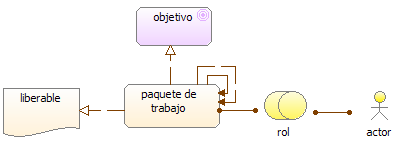
\includegraphics[scale=0.2]{figuras/23}
	\captionsetup{width=.95\textwidth}
	\caption{Posición del punto de vista de infraestructura conceptual y marco del punto de vista}
	\label{figura23}
  \end{figure}

  \subsection{Metamodelo}
  El metamodelo de la Figura 8.3 se centra en los nodos y los componentes, se muestra como las piezas de software están contenidas en los recursos físicos.

  \begin{figure}[H]
	\centering
	\includegraphics{metamodelos/11}
	\captionsetup{width=.95\textwidth}
	\caption{Metamodelo punto de vista de infraestructura}
	\label{metamodelo11}
  \end{figure}

  \subsection{Modelo mInstituto}
  La infraestructura para el aplicativo mInstituto esta basada en un portal comercial el cual necesitara de un hosting de bajo costo que a su vez lleve la menor cantidad de soporte a nivel de seguridad y actualizaciones que no van mas allá de noticias. Por otro lado tenemos nuestro portal para el aplicativo, este estará hospedado en un proveedor de servicios que responda con las necesidades de base de datos asi como la demanda de consulta de todos los modulós. La comunicación sera a través de Internet de un proveedor de servicios contratado por el cliente.
  
  \begin{figure}[H]
	\centering
	\includegraphics[scale=0.7]{modelos/11}
 	\captionsetup{width=.95\textwidth}
	\caption{Modelo punto de vista de infraestructura: minstituto}
	\label{modelo11}
  \end{figure}
  
  \section{Punto de Vista Uso de Infraestructura}
  El punto de vista de uso Infraestructura muestra cómo las aplicaciones son compatibles con el software y hardware de infraestructura: los servicios de infraestructura son entregados por los dispositivos; el software y redes de sistema se proporcionan a las aplicaciones. Este punto de vista desempeña un papel importante en el análisis de rendimiento y escalabilidad, puesto que se refiere la infraestructura física para el mundo lógico de aplicaciones. Es muy útil en la determinación de los requisitos de rendimiento y calidad en la infraestructura basada en las exigencias de las diferentes aplicaciones que lo utilizan.
  
  \begin{table}[H]
  	\centering
  	\begin{tabular}{lp{8cm}}
  		\toprule
  		\textbf{Nombre} & \textbf{Uso de la infraestructura} \\
  		\midrule
  		\textbf{Stakeholders} & Arquitectos de infraestructura y aplicación, gerentes de operación \\
  		\textbf{Preocupaciones} & Dependencias, escalabilidad y rendimiento \\
  		\textbf{Propósito} & Diseñar \\
  		\textbf{Nivel de Abstracción} & Coherencia \\
  		\textbf{Capa} & Capa de Aplicación y Tecnología \\
  		\textbf{Aspectos} & Activo, (comportamiento) \\
  		\bottomrule
  	\end{tabular}
  	\captionsetup{width=.95\textwidth}
  	\caption{Descripción punto de vista uso de infraestructura}
  	\label{tabla15}
  \end{table}
  
  \begin{figure}[H]
  	\centering
  	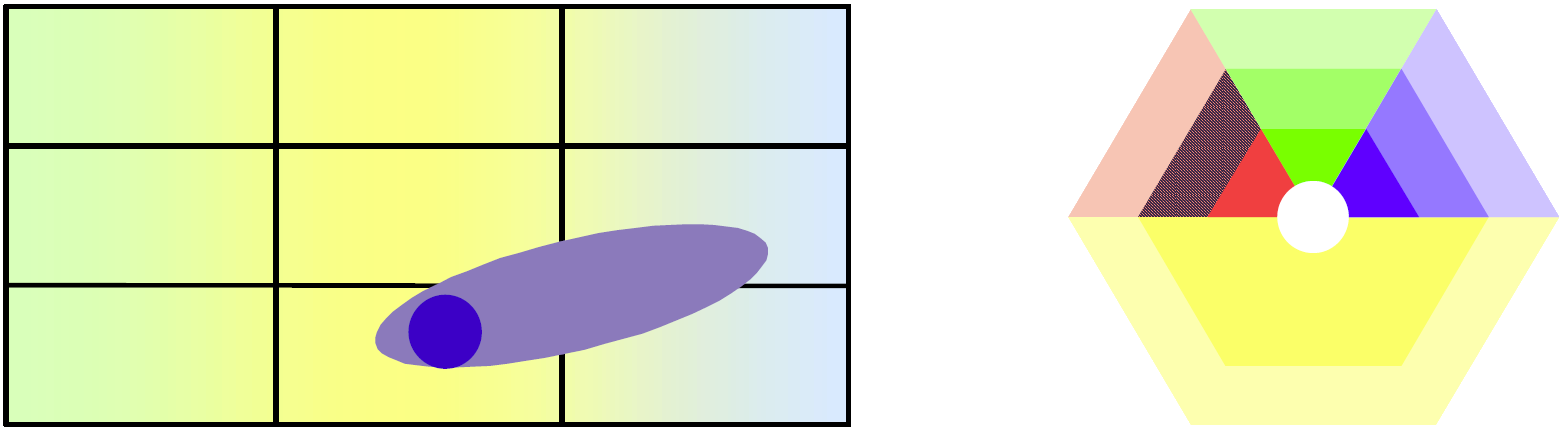
\includegraphics[scale=0.2]{figuras/24}
  	\captionsetup{width=.95\textwidth}
  	\caption{Posición del punto de vista uso de infraestructura conceptualmente y marco del punto de vista}
  	\label{figura24}
  \end{figure}
  
  \subsection{Metamodelo}
  El metamodelo de la Figura 8.3 se centra en los nodos y los componentes, se muestra como las piezas de software están contenidas en los recursos físicos.
  
  \begin{figure}[H]
  	\centering
  	\includegraphics{metamodelos/12}
  	\captionsetup{width=.95\textwidth}
  	\caption{Metamodelo punto de vista uso de infraestructura}
  	\label{metamodelo12}
  \end{figure}
  
  \subsection{Modelo mInstituto}
  El servidor de la página web está destinado a la parte comercial de la empresa, tiene como principales componentes la administración de parte de las estrategias de mercadeo y publicidad y por otro lado se encuentra el acceso a una comunidad basada en redes sociales; este a su vez se comunica con el servidor de aplicaciones a través del punto de acceso o pantalla de login donde nuestros clientes accederán a la aplicación de Minstituto.com, el aplicativo posee herramientas de accesibilidad para los usuarios y perfiles autorizados y tiene incluido un módulo de transacciones y pagos el cual cuenta con el nivel de seguridad informática acorde a las necesidades de la información
  
  \begin{figure}[H]
  	\centering
  	\includegraphics[scale=0.7]{modelos/12}
  	\captionsetup{width=.95\textwidth}
  	\caption{Modelo punto de vista uso de infraestructura: minstituto}
  	\label{modelo12}
  \end{figure}
  
  \section{Punto de Vista de Organización e implementación}
  La aplicación y el punto de vista de implementación muestran cómo una o más aplicaciones se realizan o se colaboran dentro de la infraestructura, como las aplicaciones son soportadas por el software y el hardware de infraestructura, los servicios de infraestructura son entregados por los dispositivos; el software y las redes del sistema se proporcionan a las aplicaciones, este punto de vista desempeña un papel importante en el análisis de rendimiento y escalabilidad y que hacer referencia a la infraestructura física para el mundo
  lógico.
  
  \begin{table}[H]
  	\centering
  	\begin{tabular}{lp{8cm}}
  		\toprule
  		\textbf{Nombre} & \textbf{Organización e Implementanción} \\
  		\midrule
  		\textbf{Stakeholders} & Arquitectos de infraestructura y aplicación gerente de operación \\
  		\textbf{Preocupaciones} & Dependencias, seguridad, riesgos \\
  		\textbf{Propósito} & Diseñar \\
  		\textbf{Nivel de Abstracción} & Coherencia \\
  		\textbf{Capa} & Capa de tecnología, capa de aplicación \\
  		\textbf{Aspectos} & Activo (Comportamiento) \\
  		\bottomrule
  	\end{tabular}
  	\captionsetup{width=.95\textwidth}
  	\caption{Descripción punto de vista de organización e implementación}
  	\label{tabla16}
  \end{table}
  
  \begin{figure}[H]
  	\centering
  	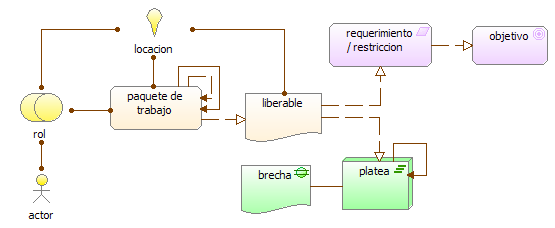
\includegraphics[scale=0.2]{figuras/25}
  	\captionsetup{width=.95\textwidth}
  	\caption{Posición de la organización e implementación conceptualmente y marco del punto de vista}
  	\label{figura25}
  \end{figure}
  
  \subsection{Metamodelo}
  En el metamodelo de la Figura 8.5 se aprecia como los diferentes nodos de infraestructura que contienen los componentes de aplicación soportan las comunicación entre ellos, muestran como componen elementos de colaboración los cuales permiten tener sistemas de cruce entre sistemas y componentes de aplicación. En el metamodelo se aumenta un componente de infraestructura para reflejar el concepto de colaboración.
  
  \begin{figure}[H]
  	\centering
  	\includegraphics{metamodelos/13}
  	\captionsetup{width=.95\textwidth}
  	\caption{Metamodelo punto de vista de organización e implementación}
  	\label{metamodelo13}
  \end{figure}
  
  \subsection{Modelo mInstituto}
  En este punto de vista observamos que Minstituto.com utiliza un servidor Linux y sobre este se ejecuta el código Java utilizando su máquina virtual y conectado a una base de datos postgreSQL. \\
  
  Para el portal comercial tendremos en un hosting compartido, una página web elaborada en PHP con una base de datos MySQL. Las dos podrán ser consultadas por los clientes usando Internet de sus proveedor de servicios y un navegador que soporte lenguaje HTML en su última versión, así como tener habilitado la ejecución de código javascript para validaciones necesarias en ambos portales.

  \begin{figure}[H]
  	\centering
  	\includegraphics[scale=0.7]{modelos/13}
  	\captionsetup{width=.95\textwidth}
  	\caption{Modelo punto de vista de organización e implementación: minstituto}
  	\label{modelo13}
  \end{figure}

\section{Punto de Vista de Estructura de Información}
El punto de vista de estructura de información es comparable a los modelos tradicionales de información creados en el desarrollo de casi cualquier sistema de información. Se muestra la estructura de la información utilizada en la empresa o en un proceso de negocio específico o aplicación, en términos de tipos de datos o las estructuras de clase (orientada a objetos). Además, puede mostrar cómo se representa la información a nivel
de empresa (objetos de negocio), a nivel de aplicación en forma de estructuras de datos utilizadas (objetos de datos), y cómo éstos se asignan a la infraestructura subyacente; por ejemplo por medio de un esquema de base de datos (artefacto).
    
    \begin{table}[H]
    	\centering
    	\begin{tabular}{lp{8cm}}
    		\toprule
    		\textbf{Nombre} & \textbf{Estructura de la información} \\
    		\midrule
    		\textbf{Stakeholders} & Arquitectos de dominio e información \\
    		\textbf{Preocupaciones} & Estructura, dependencias e inconsistencia del uso de los datos y la información  \\
    		\textbf{Propósito} & Diseñar \\
    		\textbf{Nivel de Abstracción} & Detalle \\
    		\textbf{Capa} & Capa de negocio, capa de tecnología, capa de aplicación \\
    		\textbf{Aspectos} & Pasivo \\
    		\bottomrule
    	\end{tabular}
    	\captionsetup{width=.95\textwidth}
    	\caption{Descripción punto de vista de estructura de información}
    	\label{tabla17}
    \end{table}
    
    \begin{figure}[H]
    	\centering
    	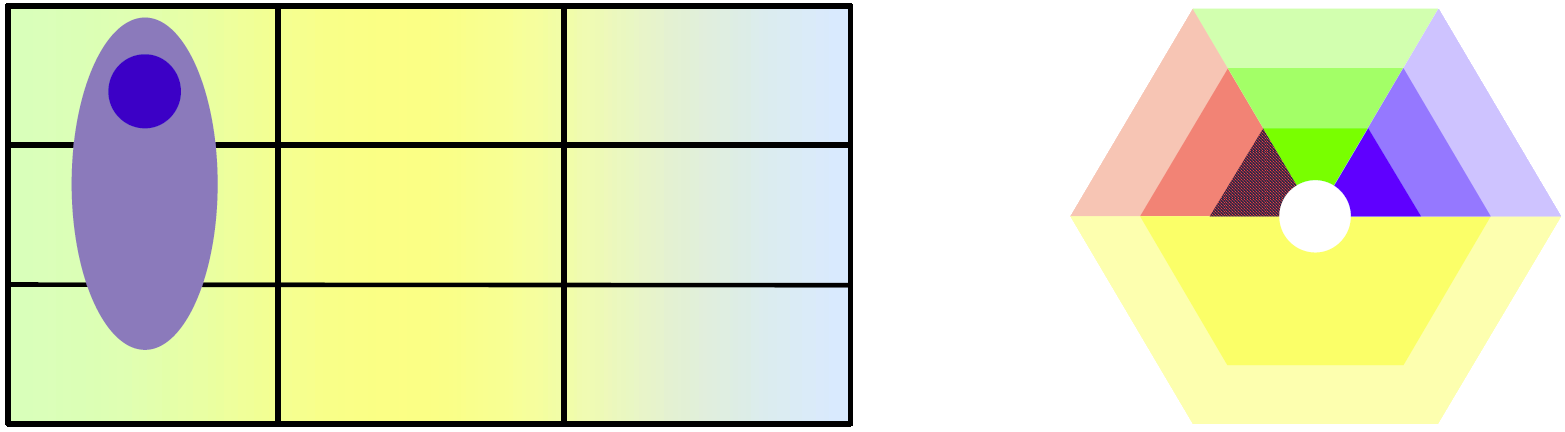
\includegraphics[scale=0.2]{figuras/26}
    	\captionsetup{width=.95\textwidth}
    	\caption{Posición del punto de vista de estructura de información conceptualmente y marco del punto de vista}
    	\label{figura26}
    \end{figure}
    
    \subsection{Metamodelo}
    El metamodelo del punto de vista de estructura de información Figura 8.7 da una buena pista de cómo se modelan los elementos finales del negocio que empezamos a percibir, el objeto de negocios el cual baja a un objeto de datos el cual nosotros llamamos artefacto en la infraestructura, le podemos asociar representaciones. El metamodelo es un sistema de conceptos que constituye un sistema de información.
    
    \begin{figure}[H]
    	\centering
    	\includegraphics{metamodelos/14}
    	\captionsetup{width=.95\textwidth}
    	\caption{Metamodelo punto de vista de estructura de información}
    	\label{metamodelo14}
    \end{figure}
    
    \subsection{Modelo mInstituto}
    El manejo de información estará basado en el producto, este tendrá el manejo de comercialización y toda la parte de mercadeo entregando al cliente solo lo que impacte y genere en él una decisión de compra. Capacitación: brindar todas las herramientas necesarias para que se pueda hacer un uso correcto de la herramienta y que nos limite al máximo toda la parte de soporte post-venta. Documentación: mantener al día los manuales de usuario con nuevas funcionalidades así como nuevos desarrollos, tips y ayuda para cada una de la pantallas de la plataforma.
    
    \begin{figure}[H]
    	\centering
    	\includegraphics[scale=0.65]{modelos/14}
    	\captionsetup{width=.95\textwidth}
    	\caption{Modelo punto de vista de estructura de información: minstituto}
    	\label{modelo14}
    \end{figure}
    
\section{Punto de vista de realización del servicio}
El punto de vista de realización del servicio es usado para mostrar como uno o mas servicios de negocio son realizados por los procesos subyacentes(y algunas veces por componentes de aplicación). Así, se forma el puente entre el punto de vista de producto de negocio y la vista de proceso de negocio. Proporciona una "vista desde afuera" sobre uno o mas procesos de negocio.
    
    \begin{table}[H]
    	\centering
    	\begin{tabular}{lp{8cm}}
    		\toprule
    		\textbf{Nombre} & \textbf{Realización del servicio} \\
    		\midrule
    		\textbf{Stakeholders} & Proceso y de dominio, arquitectos y gerentes de producto operativos \\
    		\textbf{Preocupaciones} & Valor añadido de los procesos de negocio, Coherencia e integridad,
    		responsabilidades \\
    		\textbf{Propósito} & Diseñar, Decidir \\
    		\textbf{Nivel de Abstracción} & Coherencia \\
    		\textbf{Capa} & Capa de Negocios (Aplicación) \\
    		\textbf{Aspectos} & Comportamiento, estructura, información \\
    		\bottomrule
    	\end{tabular}
    	\captionsetup{width=.95\textwidth}
    	\caption{Descripción punto de vista de realización del servicio}
    	\label{tabla18}
    \end{table}
    
    \begin{figure}[H]
    	\centering
    	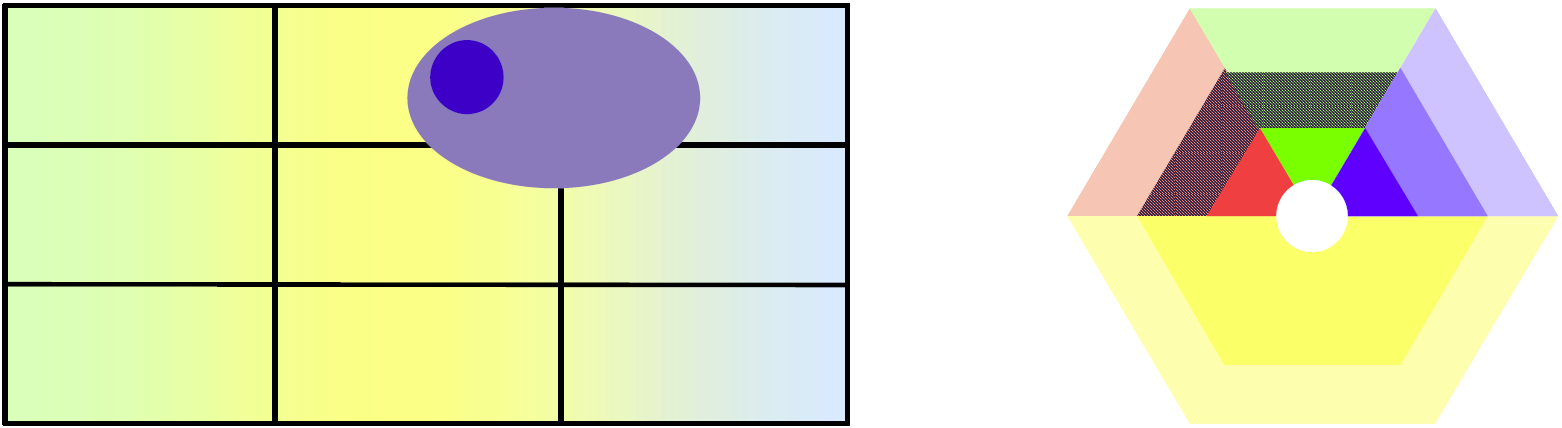
\includegraphics[scale=0.2]{figuras/27}
    	\captionsetup{width=.95\textwidth}
    	\caption{Posición del punto de vista de realización del servicio conceptualmente y marco del punto de vista}
    	\label{figura27}
    \end{figure}
    
    \subsection{Metamodelo}
    El metamodelo del punto de vista de estructura de realización del servicio nos muestra cómo se modelan los elementos finales del negocio que empezamos a percibir, sus competencias al igual que las responsabilidades basado en la estructura y la información.
    
    \begin{figure}[H]
    	\centering
    	\includegraphics{metamodelos/15}
    	\captionsetup{width=.95\textwidth}
    	\caption{Metamodelo punto de vista de estructura de realización del servicio}
    	\label{metamodelo15}
    \end{figure}
    
    \subsection{Modelo mInstituto}
    En este modelo se presenta el producto que obtiene el cliente luego de un licenciamiento. Como punto de partida tenemos la comercialización que iniciará con una orden de compra y la aceptación de los términos y condiciones de uso de la plataforma, el cliente recibirá mes a mes su facturación a través del gestor contable. Software: MInstituto con todas las funcionalidades descritas en los términos y condiciones. Soporte: esa necesidad vital del ciclo del software que permite al aplicativo crecer por medio de la retroalimentación y generar comunicación y confianza de nuestros clientes a través de un excelente servicio post-venta, manejado por un gestor de clientes que recibirá todas las solicitudes en diferentes escalas y serán gestionadas por nuestros profesionales de las diferentes áreas.
    
    \begin{figure}[H]
    	\centering
    	\includegraphics[scale=0.65]{modelos/15}
    	\captionsetup{width=.95\textwidth}
    	\caption{Modelo punto de vista de estructura de realización del servicio: minstituto}
    	\label{modelo15}
    \end{figure}

\section{Punto de Vista de Capas}
El punto de vista de capas ilustra en un diagrama de capas los aspectos de una arquitectura
empresarial. Hay dos categorías de capas, capa dedicada y capa de servicios. Las capas
son el resultado de la utilización de la relación “agrupación” de todo el conjunto de objetos
y relaciones que pertenecen a un modelo. La infraestructura, la aplicación, el proceso
y los actores / roles pertenecen a la categoría de capa dedicada. La Tabla 8.5 describe el
punto de vista.
    
  \begin{table}[H]
  	\centering
   	\begin{tabular}{lp{8cm}}
   		\toprule
   		\textbf{Nombre} & \textbf{Vista de Capas} \\
   		\midrule
   		\textbf{Stakeholders} & Arquitectos de Organización, proceso, aplicación, infraestructura y dominio \\
   		\textbf{Preocupaciones} & Consistencia, reducción de la complejidad, impacto del cambio y flexibilidad \\
   		\textbf{Propósito} & Diseñar, decidir, informar \\
   		\textbf{Nivel de Abstracción} & Información General \\
   		\textbf{Capa} & Capa de Negocio, Capa de Tecnología, Capa de Aplicación \\
   		\textbf{Aspectos} & Activo, comportamiento, pasivo \\
   		\bottomrule
   	\end{tabular}
   	\captionsetup{width=.95\textwidth}
   	\caption{Descripción punto de vista de capas}
   	\label{tabla19}
  \end{table}
    
  \begin{figure}[H]
   	\centering
   	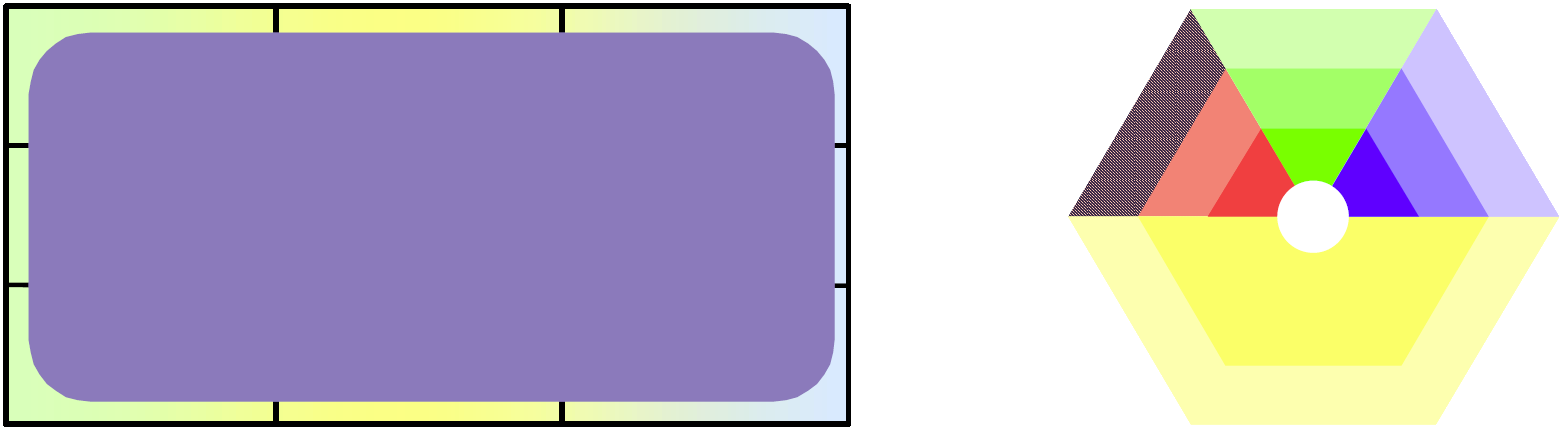
\includegraphics[scale=0.2]{figuras/28}
   	\captionsetup{width=.95\textwidth}
   	\caption{Posición del punto de vista de capas conceptualmente y marco del punto de vista}
   	\label{figura28}
   \end{figure}
   
   \subsection{Metamodelo}
   El metamodelo Figura 8.9 expresa la conexión entre las capas por medio de los servicios o de los componentes que integran a cada una, la capa de infraestructura se relaciona por medio del servicio de aplicaciones con el componente de aplicación de la capa de aplicación, este componente a su vez se relaciona con el proceso de negocio de la capa de negocio y por ultimo este proceso de negocio se relaciona con los servicio de negocio de la organización.
  
   \begin{figure}[H]
   	\centering
   	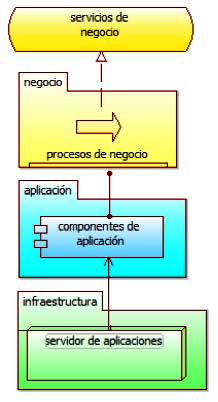
\includegraphics{metamodelos/16}
   	\captionsetup{width=.95\textwidth}
   	\caption{Metamodelo punto de vista de capas}
   	\label{metamodelo16}
   \end{figure}
   
   \subsection{Modelo mInstituto}Chachara del diagrama
   \begin{figure}[H]
   	\centering
   	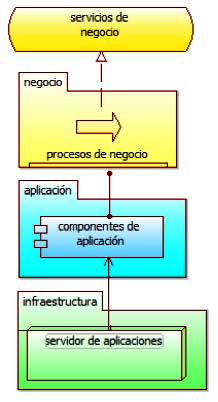
\includegraphics{metamodelos/16}
   	\captionsetup{width=.95\textwidth}
   	\caption{Modelo punto de vista de capas: minstituto}
   	\label{modelo16}
   \end{figure}